\documentclass[12pt,a4paper]{article}

\usepackage[hidelinks]{hyperref}

\usepackage[pdftex]{graphicx}

\usepackage{titlesec}

\usepackage{array}

\newcommand{\HRule}{\rule{\linewidth}{0.5mm}}

\setcounter{secnumdepth}{5}

\titleformat{\paragraph}
{\normalfont\normalsize\bfseries}{\theparagraph}{1em}{}

\titlespacing*{\paragraph}
{0pt}{3.25ex plus 1ex minus .2ex}{1.5ex plus .2ex}

\hyphenation{my-Ta-xi-Ser-vi-ce}

\begin{document}
	\begin{titlepage}
\begin{center}

% Upper part of the page. The '~' is needed because \\
% only works if a paragraph has started.

%we can put here the polilogo
~\\[1cm]

\includegraphics[width=0.28\textwidth]{./logo-polimi}~\\[1.5cm]

\textsc{\huge \textsc{Software Engineering 2}
}
\\[1cm]

% Title
\HRule \\[0.4cm]
{ \huge \bfseries Requirement Analysis and Specification Document\\
		(RASD) \\[0.3cm]
		}
\HRule \\[1.5cm]

% Author
\noindent
\begin{minipage}{1.0\textwidth}
\begin{center}


\textsc{\large{Authors}} \\
\large{
Paolo Paterna, Lara Premi \\
\vspace{0.8cm}
\small{
Politecnico di Milano, Italy\\
Email: paolo.paterna@mail.polimi.it, lara.premi@mail.polimi.it
}
}

\end{center}
\end{minipage}%

\vfill
% Bottom of the page
\textbf{\large{6th Nov 2015}}

\end{center}
\end{titlepage}
	\tableofcontents
	\newpage
	\section{Introduction}
\subsection{Purpose}
	This document is the Design Document (DD) of a system, called myTaxiService, used to manage  a taxi service in a city. The main goals of this document is to specify how the system has to be build in terms of software and hardware architecture, focusing on how the software architecture is built, what kind of styles are used and which kind of tiered architecture is used for the hardware part.
\subsection{Scope}
	The scope of this system is to manage taxis in a city. A town is divided in zone of 2 square kilometers and, for each zone, the system defines a queue, composed by the identifier, which is the vehicle plate, of free taxis in that specific zone. A user can require a taxi ride from a zone, but he/she can also book one for another moment, using the web application or the mobile one. Furthermore, about long-term reservations, after the user has created one, he/she is able to modify the date or the hour or both of his/her booking, and he/she can delete it. 
\subsection{Definitions, acronyms and abbreviations}
	\subsubsection{Definitions}
	\subsubsection{Acronyms}
		 \begin{itemize}
		 	\item RASD: Requirements Analysis and Specification Document from previous delivery
		 \end{itemize}
	\subsubsection{Abbreviations}
		\begin{itemize}
			\item Gi: goal number i, that refers to the corresponding goal in the RASD.
		\end{itemize}
\subsection{Reference Documents}
	To redact this document, we used the following other documents as references:
	\begin{itemize}
		\item Requirements Analysis and Specification Document from previous delivery
		\item Design Document Table of Content 
	\end{itemize}
\subsection{Document Structure}
	This document contains the schema that represents the software and the hardware architectures, the sequence diagrams that show how the system works and the design choices made to build the system. After that, there are some implementations in pseudo code, user interfaces and all the requirements present in the RASD, mapped in this document.
	\section{Architectural Design}
\subsection{Overview}
	
\subsection{High level components and their interaction}
\subsection{Component view}
	\begin{center}
		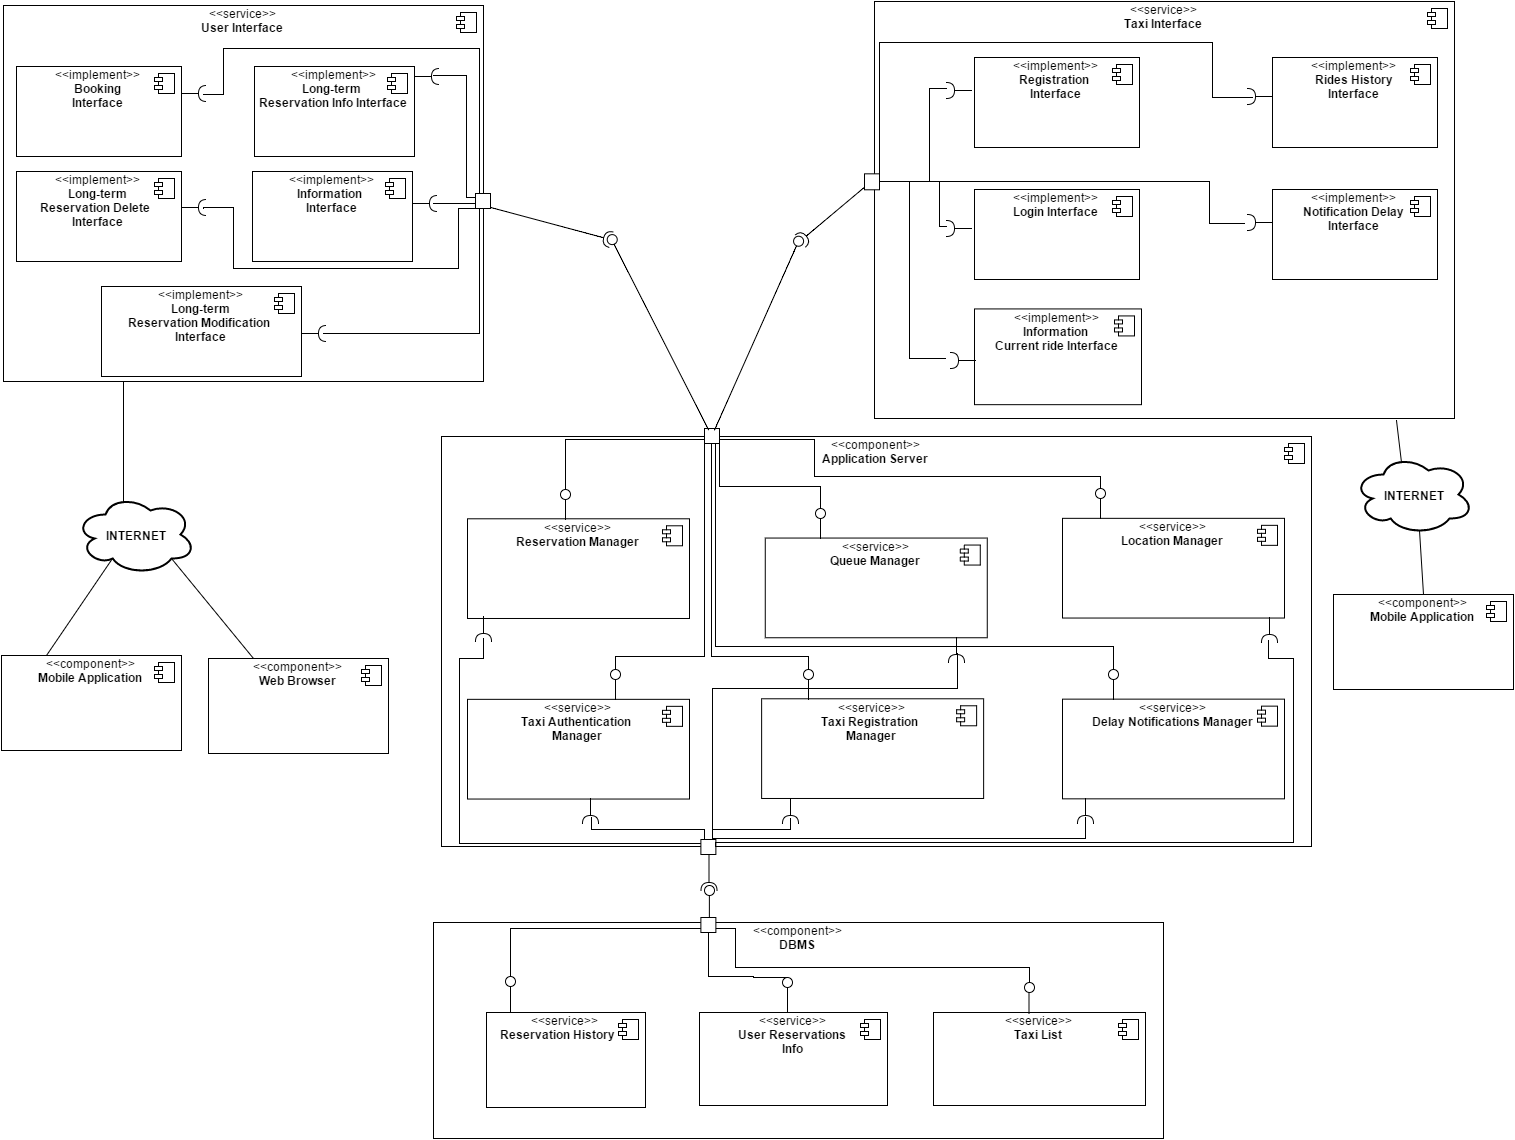
\includegraphics[width=0.95\textwidth]{./images/component_view.png}
	\end{center}
	
\subsection{Deployment view}
	\begin{center}
		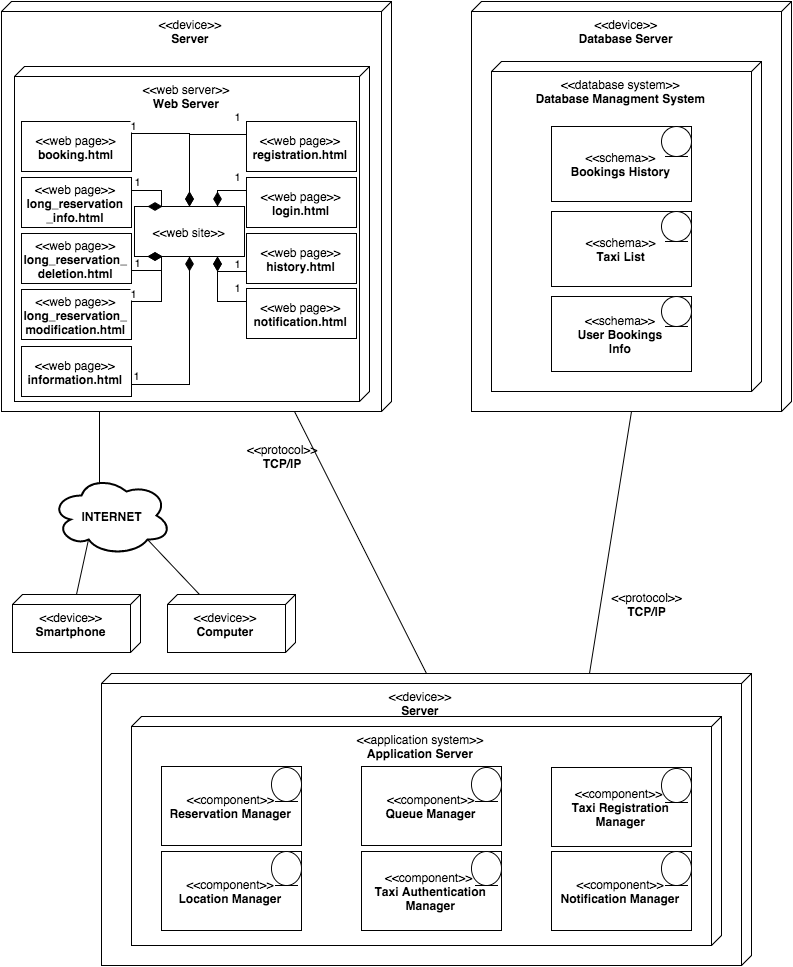
\includegraphics[width=0.95\textwidth]{./images/deployment_view.png}
	\end{center}
\subsection{Runtime view}
\subsection{Component interfaces}
\subsection{Selected architectural styles and patterns}
\subsection{Other design decisions}
	\subsubsection{Design patterns}
	\section{Algorithm Design}
\subsection{Queue manager}
\begin{algorithmic}
	\Function{manageQueue}{zone}
		\State $queue\gets getZoneQueue(zone)$
		\While{queueIsEmpty}
				\State $adjacentZone \gets getAdjacentZone(zone)$
				\State $queue\gets getZoneQueue(adjacentZone)$
		\EndWhile
		\State $taxiCode \gets getTaxi(queue)$
		\State \Return{$taxiCode$}
	\EndFunction
\end{algorithmic}
\subsection{Reservation Manager}
\begin{algorithmic}
	\Function{manageBooking}{location, time, destination}
		\If {$!locationIsValid(location)  \&\& !timeIsValid(time)$} 
			\State \Return error 
		\EndIf
		\If{$time = CURRENT \textunderscore TIME$}
			\State $reservation \gets createShortReservation(location, destination)$
			\State $zone \gets getZone(location)$
			\While{!positiveResponse}
				\State $taxi \gets manageQueue(zone)$
				\State $response \gets jobNotification(taxi)$
			\EndWhile	
		\Else 
			\State $reservation \gets createLongReservation(location, time, destination)$
			\State $saveReservation(reservation, database)$
			\State \Return
		\EndIf
		\State $sendConfirmation(reservation)$
		\State \Return
	\EndFunction
\end{algorithmic}
	\section{User Interface Design}
	\section{Requirements Traceability}
The list above shows how the goals, defined in the RASD, are mapped into the design elements, that we have defined in the upper sections of this document.
\newline
\newline
	\emph{G1}
		\begin{itemize}
			\item Using the smartphone or the computer, the user clicks on the button, that lets him/her to book a ride.
			\item The web server loads the web page "user reservation.html".
			\item The user can view the booking interface and he/she can ask to a ride.
			\item Through the TCP/IP protocol, the web server sends the information, inserted by the user, to the application server.
			\item The application server, using the reservation manager and thanks to the TCP/IP protocol, executes an SQL query with the user's information to the DBMS.
			\item The DBMS saves these information in the specific table "User Reservation Info".
		\end{itemize}
	\emph{G2}
		\begin{itemize}
			\item Using the smartphone or the computer, the user clicks on the button, that lets him/her to modify the date and/or the hour of his/her long-term reservation.
			\item The web server loads the web page "reservation modification.html".
			\item The user can view the long-term reservation modification interface and he/she can ask to modify his/her ride.
			\item Through the TCP/IP protocol, the web server sends the information, inserted by the user, to the application server.
			\item The application server, using the reservation manager and thanks to the TCP/IP protocol, executes an SQL query with the user's information to the DBMS.
			\item The DBMS changes the old information with the new ones, in the specific table "User Reservation Info".
		\end{itemize}
	\emph{G3}
		\begin{itemize}
			\item Using the smartphone or the computer, the user clicks on the button, that lets him/her to delete a long-term reservation.
			\item The web server loads the web page "reservation deletion.html".
			\item The user van view the long-term reservation delete interface and he/she can ask to cancel his/her ride.
			\item Through the TCP/IP protocol, the web server sends the the alphanumeric code, inserted by the user, to the application server.
			\item The application server, using the reservation manager and thanks to the TCP/IP protocol, executes an SQL query with the user' alphanumeric code to the DBMS.
			\item The DBMS deletes the long-term reservation information from the specific table "User Reservation Info".
		\end{itemize}
	\emph{G4}
		\begin{itemize}
			\item Before to accept the user's request for a booking, the application system uses the location manager.
			\item The application server, in this way, thanks to the GPS information, can check if the address, inserted by the user, is valid or not.
		\end{itemize}
	\emph{G5}
		\begin{itemize}
			\item The application server uses the location manager.
			\item In this way, the application server, thanks to the GPS information, identifies the current position of the taxi.
		\end{itemize}
	\emph{G6}
		\begin{itemize}
			\item After the identification of the taxi position, the application server uses the queue manager to understand which is the queue relative to the zone where there is the taxi in this moment.
			\item The application server inserts the taxi identifier, that is the vehicle plate, in this zone's queue, if the taxi is free.
			\item The application server deletes the taxi identifier, that is the vehicle plate, from this zone's queue, if the taxi is not yet available.
			\item The application server assigns to the first taxi in the queue the request of a user, if he/she has requested a taxi in this zone.
			\item If the zone's queue is empty, the application server, through the location manager, checks which four zones are adjacent of the requested zone. Then, the application server does the same things, already described previously.
		\end{itemize}
	\emph{G7}
		\begin{itemize}
			\item Using the smartphone, the new taxi clicks on the button, that lets him/her to register in the system.
			\item The web server loads the web page "registration.html".
			\item The new taxi can view the registration interface.
			\item Through the TCP/IP protocol, the web server sends the information, inserted by the new taxi, to the application server.
			\item The application server, using the taxi registration manager and thanks to the TCP/IP protocol, executes an SQL query with the new taxi's information to the DBMS.
			\item The DBMS inserts these information in the specific table "Taxi List".
		\end{itemize}
	\emph{G8}
		\begin{itemize}
			\item The application server, using the notification manager, sends an SMS, after the user changed his/her long-term reservations.
		\end{itemize}
	\emph{G9}
		\begin{itemize}
			\item The application server uses the location manager and, thanks to the GPS information, it identifies the position of the user.
			\item The application server sends a notification to the first taxi available in the queue of the zone, from where the user has requested a taxi.
		\end{itemize}
		
		
		
		
		
		
		
		
		
		
		
		
		
		
		
		
		
		
		
		
		
		
		
		
		
		
		
		
		
		
		
		
		
	\newpage
	\section{References}
	\begin{itemize}
		\item Requirements Analysis and Specification Document from previous delivery;
		\item Design Document Table of Content;
		\item Slides "Software architectures and styles.pdf" of professor Tamburri;
		\item Draw.io \url{http://www.draw.io} to draw component view diagram and deployment view diagram;
		\item Web Sequence Diagram \url{http://www.websequencediagrams.com/} to draw the sequence diagrams. 
	\end{itemize}
	
\end{document}